\documentclass[UTF8,11pt,fontset=fandol]{ctexart}
\usepackage[margin=1in]{geometry}
\usepackage{graphicx}
\usepackage{booktabs}
\usepackage{multirow}
\usepackage{amsmath,amssymb}
\usepackage{xcolor}
\usepackage{hyperref}
\usepackage{enumitem}
\usepackage{subcaption}
\usepackage{tikz}
\usetikzlibrary{arrows.meta,positioning,fit}
\hypersetup{colorlinks=true,linkcolor=blue,citecolor=blue,urlcolor=blue}

\title{面向多模态几何推理的 Compact Theorem Routes\\
\large 中间几何语言的选择性暴露}
\author{Anonymous Authors}
\date{2026 年 6 月}

\begin{document}
\maketitle

\begin{abstract}
中间几何语言通常被视为多模态大模型（MLLM）的辅助上下文：解析题图，追加符号事实，再让 MLLM 解题。本文提出选择性暴露视角：第一，描述性结构本身不是可靠干预；第二，compact theorem route 更强，因为它把图形解析压缩成定理级行动；第三，真正关键的不是 route 格式本身，而是 route 在暴露前是否经过筛选和信任校准。基于 Geometry3K、PGPS9K 和 GeoQA 的实验显示，GDP-style 结构事实和未筛选 oracle predicates 都可能无法提升 raw image solving。相比之下，定理路线本身有价值：在 GeoQA271 上，generated route guidance 将 Qwen3-VL-8B 从 30.63\% 提升到 38.01\%，verified-policy route 达到 40.59\%。FormalGeo oracle-route 检查将 29.00\% 提升到 41.50\%，但由于 FormalGeo 与 GeoQA 的难度和标注格式不同，本文仅将其作为定性 sanity check。关键问题转向校准：在同一个 GeoQA271 划分上，verified-policy route 仍然最好，而 equation 和 hybrid candidates 优于 direct route。这支持一个级联策略：优先筛选 route；当 route 置信度不足时，把它降级为目标绑定的 theorem-equation candidates；如果置信度仍低，则退回 raw image solving。我们还发现 compact route 可以为小型 VLM 提供推理时定理规划辅助：InternVL3-2B 从 15.75\% 提升到 31.75\%，而强 8B 模型收益较小。
\end{abstract}

\section{引言}
图形几何推理是多模态模型的高密度压力测试：模型必须识别几何实体，绑定标签与数量，选择适用定理，并计算目标值。因此，经典 neuro-symbolic 系统通常会先将题图和文本转成 formal language，再进行求解。Inter-GPS 将几何题解析为形式化表示并进行可解释推理 \cite{lu2021intergps}；GeoQA 提出了面向几何数值推理的多模态问答基准 \cite{chen2021geoqa}；FormalGeo 系统化组织几何条件、定理序列和可验证求解轨迹 \cite{zhang2023formalgeo}；DFE-GPS 和 Geoparsing 等近期工作进一步面向 MLLM 时代重新研究图形形式化与统一形式语言解析 \cite{zhang2024dfegps,wang2026geoparsing}。

这些工作自然引出一个假设：如果 MLLM 在原图之外还能看到结构化几何描述，解题准确率应该提高。我们的实验说明，这个假设并不完整。中间语言不是被动上下文，而是对模型推理轨迹的干预。一个看似正确的结构事实可能与目标量无关；一条定理路线可能使用真实定理，却服务于错误子问题；一个过于权威的 route 还可能覆盖模型本来正确的视觉判断。因此，核心问题不是“是否给中间语言”，而是\emph{暴露什么数学单元，以及在什么可靠性条件下暴露}。

本文研究三个逐渐接近解题动作的单元：\emph{结构事实}、\emph{紧凑定理路线}和\emph{定理-方程候选}。实验证据显示出清晰层次：结构事实往往不够，因为它只描述“看见了什么”，没有描述“应该怎么做”；compact route 更强，因为它把解析结果压缩成定理级行动；定理-方程候选并不是为了替代 verified route，而是在 route 级验证不可靠时，把 route 转换成目标绑定、前提可检查的小规模选择问题。

本文的贡献如下：
\begin{itemize}[leftmargin=*]
\item \textbf{给出无条件结构暴露的反例。} 我们展示 GDP-style 自动结构和未筛选 oracle predicates 在作为普通上下文追加时，都可能无法提升 Qwen3-VL-8B。
\item \textbf{把 compact route 定位为定理级压缩和规划辅助。} 我们展示 generated route 可以把图形解析压缩为面向目标的定理行动，并在 GeoQA 与跨模型 PGPS9K+Geometry3K 测试中提升下游 MLLM 解题准确率，尤其对较小 VLM 更明显。
\item \textbf{用 win--loss 视角分析 route 可靠性。} 我们不只报告 accuracy，而是统计 route 相对 raw image solving 修正了多少错误、又破坏了多少原本正确的答案。
\item \textbf{提出选择性暴露级联。} 系统应先验证 route 可靠性；若验证不足，再将 route 降级为 theorem-equation candidate；若仍不可信，则隐藏中间语言。
\end{itemize}

\section{作为数学接口的中间语言}
本文不是简单替换 prompt 模板。核心问题是上游解析器或 route generator 与下游 MLLM 之间的计算契约。三类中间语言承担不同数学角色：

\begin{itemize}[leftmargin=*]
\item \textbf{结构化事实}描述图中有什么：点、线、角度、平行、垂直、切线等关系。
\item \textbf{定理路线}描述可能怎么做：应该用哪些几何事实、按什么大致顺序使用。
\item \textbf{候选定理-方程}同时暴露候选 theorem binding 和可执行 方程骨架，迫使模型选择前提与目标和已知条件匹配的规则。
\end{itemize}

候选式界面更接近 formal solver 中的 theorem application：定理只有在前提能匹配到已知事实、结论又连接到目标量时才应被使用。这个视角解释了为什么某些 route 即使提到真实定理，仍然会误导模型：定理真实性弱于目标有用性。不过，同划分实验也说明 verified route 当前强于 candidate 转换本身；因此 candidates 应被理解为不确定 route 的安全降级方案，而不是 verification 的替代品。

\begin{table}[t]
\centering
\caption{中间几何语言的三层接口层级。本文并不是说后一层完全替代前一层，而是每一层都针对上一层的具体失败模式。}
\label{tab:interface-hierarchy-zh}
\small
\begin{tabular}{p{0.21\linewidth}p{0.25\linewidth}p{0.26\linewidth}p{0.18\linewidth}}
\toprule
层级 & 暴露对象 & 解决的失败模式 & 主要实验 \\
\midrule
描述性事实 & 点、线、关系等解析事实 & 补充感知，但不告诉模型怎么做 & Geometry3K 结构实验 \\
Compact route & 短定理行动序列 & 补充定理规划，但可能目标错配 & GeoQA271 与跨模型实验 \\
定理-方程候选 & 定理绑定 + 方程骨架 & route 验证较弱时的安全降级 & GeoQA220/271 candidates \\
\bottomrule
\end{tabular}
\end{table}

\begin{figure}[t]
\centering
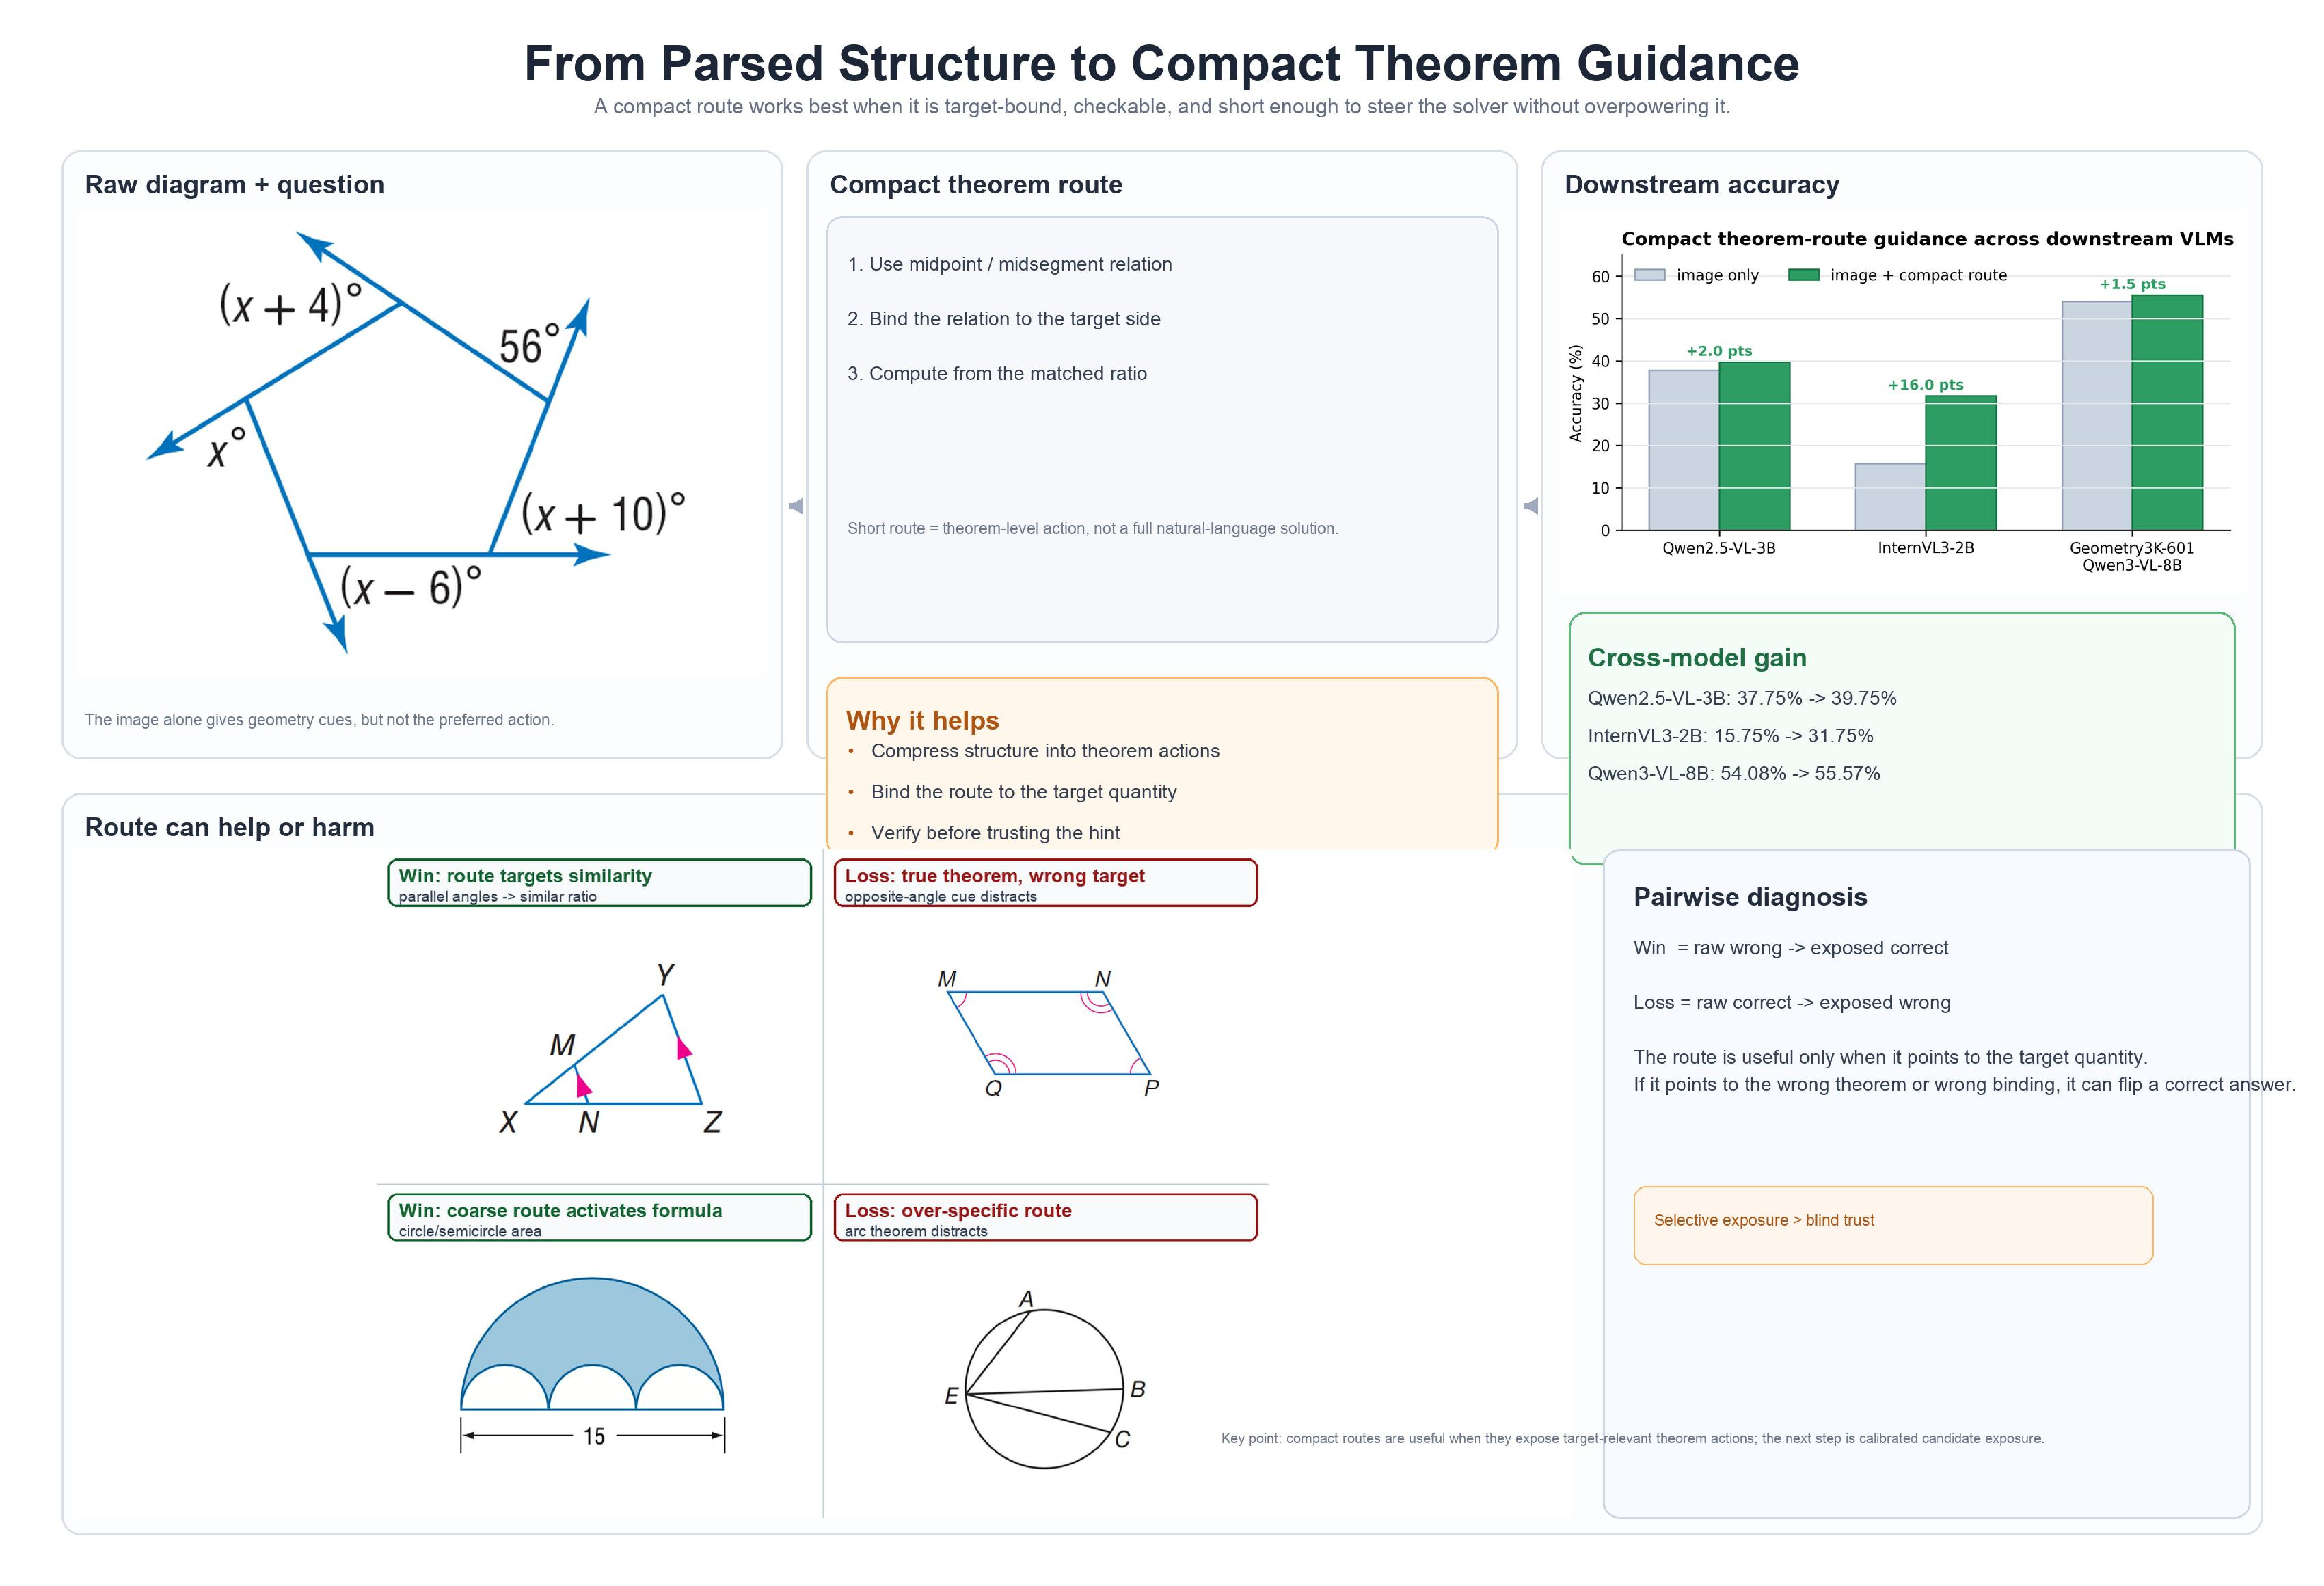
\includegraphics[width=0.98\linewidth]{figures/compact_route_core_result.pdf}
\caption{核心发现与机制。compact route 将几何解析转化为定理级行动。在多个下游设置中，image+compact-route 输入能够提升 raw image solving；但 route 必须被视为目标绑定的数学接口，而不是可信自由文本。}
\label{fig:compact-route-core-zh}
\end{figure}

\section{相关工作与问题空缺}
\paragraph{形式化几何求解。}
Inter-GPS 和 FormalGeo 等形式化求解系统强调显式几何条件、定理应用和符号验证 \cite{lu2021intergps,zhang2023formalgeo}。这些工作说明结构化数学状态对几何推理很重要。本文不同之处在于，我们不假设已经拥有完整符号求解器，而是研究部分中间语言应如何暴露给仍然读取原始图像的 MLLM。

\paragraph{几何图解析与多模态基准。}
GeoQA、Geometry3K 和 MathVista 从不同标注体系评估视觉数学推理 \cite{chen2021geoqa,lu2021intergps,lu2023mathvista}。DFE-GPS 和 Geoparsing 等近期工作提升了从图形到 formal language 的上游转换能力 \cite{zhang2024dfegps,wang2026geoparsing}。这些解析器使中间语言暴露变得更可行，但并没有回答下游 MLLM 何时应该相信这些文本。我们的实验显示，parser output 的作用取决于目标绑定和暴露策略：它可能帮助，也可能无效或有害。

\paragraph{MLLM 的中间推理接口。}
很多 MLLM 方法会通过分解、rationale、program 或 symbolic hint 改善推理。但在几何任务中，中间对象并不只是自然语言推理链，而是对应定理前提、实体绑定和方程关系。因此，盲目执行 route 特别容易带来风险。本文将中间语言视为需要校准的干预，并用 pairwise win/loss 同时衡量帮助和伤害。

\begin{table}[t]
\centering
\caption{与代表性几何和视觉数学推理工作的定位比较。已有工作主要改进解析、形式化求解、视觉语言预训练或指令微调；本文关注已经生成的中间表示何时应该暴露给 MLLM。}
\label{tab:positioning-zh}
\small
\begin{tabular}{lcccc}
\toprule
工作方向 & 形式结构 & 定理路径 & MLLM 求解 & 暴露校准 \\
\midrule
Inter-GPS / FormalGeo \cite{lu2021intergps,zhang2023formalgeo} & \checkmark & \checkmark & -- & -- \\
GDP / Geoparsing \cite{zhang2022pgdp,wang2026geoparsing} & \checkmark & -- & optional & -- \\
DFE-GPS / GeoX \cite{zhang2024dfegps,xia2025geox} & \checkmark & partial & \checkmark & -- \\
MAVIS / GeoDANO \cite{zhang2025mavis,cho2025geodano} & implicit & implicit & \checkmark & -- \\
\textbf{本文} & \checkmark & \checkmark & \checkmark & \checkmark \\
\bottomrule
\end{tabular}
\end{table}

\section{实验协议}
下游求解器使用 Qwen3-VL-8B。主要数据集是 Geometry3K \cite{lu2021intergps} 和 GeoQA \cite{chen2021geoqa}；MathVista 仅作为额外视觉数学参考 \cite{lu2023mathvista}。GDP-style 结构由几何图解析方向的 parser 生成，其方向对应 Geoparsing 等工作 \cite{wang2026geoparsing}。route 实验中，我们使用已保存的 Qwen3-1.7B LoRA generator，将结构化几何输入映射成 theorem-route 风格输出，然后再把 route 转成不同的下游接口。该 route generator 在 FormalGeo-style route data 上训练，并在 held-out 或跨数据集下游样本上评测；本文没有在用于 GeoQA 评测的样本上继续微调该 generator。

\paragraph{划分说明。}
GeoQA120、GeoQA220 和 GeoQA271 是同一个过滤后 GeoQA 顺序上的确定性前缀子集，过滤条件是答案能解析为简单数值。因此 GeoQA120 包含于 GeoQA220，GeoQA220 包含于 GeoQA271。数量不同来自实验预算和变体数量不同，而不是不同采样规则：271 题用于 route policy，120 题用于便宜地比较多种 presentation interface，220 题用于更重的 theorem-equation candidate 评测。这种嵌套关系也应被视为局限：最干净的后续比较应在同一个固定划分上运行所有接口。

评测同时报告 accuracy 和相对 raw image baseline 的 pairwise flips。win 指 raw 错、增强方法对；loss 指 raw 对、增强方法错。这个指标很关键，因为一种方法即使平均准确率提高，也可能引入新的 route-induced error。

形式化地，令 \(x_i\) 表示图像、题干和选项，\(y_i\) 表示标准答案，\(z_i\) 表示被暴露的中间对象，例如 route 或 candidate list。令 \(f_0(x_i)\) 为 raw image prediction，\(f_z(x_i,z_i)\) 为暴露中间对象后的 prediction。单题效果定义为
\begin{equation}
\Delta_i(z)=
\mathbf{1}[f_z(x_i,z_i)=y_i]-
\mathbf{1}[f_0(x_i)=y_i].
\end{equation}
其中 \(\Delta_i=1\) 是 win，\(\Delta_i=-1\) 是 loss，整体增益为
\begin{equation}
\mathrm{Gain}(z)=\frac{1}{N}\sum_i \Delta_i(z)=\frac{W(z)-L(z)}{N}.
\end{equation}
这个指标说明，即使平均增益较小，route 仍可能揭示一个高价值但校准不足的干预通道。

\paragraph{verified-policy route 的操作定义。}
本文主表中的 `verified-policy' 是轻量 route-level heuristic，而不是训练得到的 verifier。具体实现中，我们先从 route 文本中抽取 generated theorem sequence。无法抽取 theorem sequence 的 route 直接 reject；超过八步的 route，或同一个 theorem name 重复五次及以上的 route，会被标记为 low confidence。对剩余 route，我们检查 theorem family 是否匹配目标类型，以及结构化解析中是否存在对应支持谓词，例如 parallel、right-triangle 或 similar-triangle 证据。高置信 route 会连同显式 use-policy 一起暴露给 MLLM；中置信 route 会附带风险信号；低置信 route 仍可见，但只作为弱提示，要求模型优先依赖图像；reject route 则隐藏。它不同于 \emph{critique-first}：后者是在 route 已经暴露给 MLLM 后，让 MLLM 自己批判 route。后文的 strict-gate ablation 是另一套更保守的规则；其较低准确率说明硬过滤会丢掉有用信号。

在 GeoQA271 上，这个 policy 的分层结果是：high 244 题、medium 2 题、low 12 题、reject 13 题。对应的分层准确率分别是 101/244（41.39\%）、1/2（50.00\%）、7/12（58.33\%）和 1/13（7.69\%）。这些数值应只被看作操作审计，因为 medium 和 low 子集都很小。本文正文报告的 110/271 是整体验证后的加权准确率。另需说明：low-confidence 在此实验中并不等于纯 raw fallback；route 仍以弱提示形式可见，只有 reject 才完全隐藏。

\paragraph{候选转换。}
GeoQA 实验中的 theorem candidates 和 equation candidates 都不是由更强的外部 LLM 重新生成，而是从同一个 generated route source 里用确定性的规则抽取得到。我们先解析 route 中的 theorem 调用，再按出现顺序去重 theorem name，并把已知 theorem name 映射到固定的自然语言描述模板。equation candidates 则来自一组固定方程骨架模板，例如三角形内角和、平行线角相等、勾股关系、相似三角形比例以及圆中角关系。目标类型通过题干中的关键词推断，如 angle、length、area、perimeter 等。如果 route 无法解析出可用 theorem，则候选界面退回到 “none of the above / 从原图作答”。这样的设计是为了隔离暴露格式的作用，而不是引入另一模型的额外推理能力。

\begin{table}[t]
\centering
\caption{主张与证据对应表。每个核心主张都对应具体实验，并给出除 accuracy 外的诊断指标。}
\label{tab:claim-evidence-zh}
\small
\begin{tabular}{p{0.34\linewidth}p{0.34\linewidth}p{0.20\linewidth}}
\toprule
主张 & 主要证据 & 诊断指标 \\
\midrule
描述性结构并不自动有用。 & Geometry3K-300 与 Geometry3K-601 trust experiments。 & accuracy 与 raw-vs-structure flips。 \\
theorem route 能帮助，但也会破坏 raw 本来正确的答案。 & GeoQA271 route 实验和 win/loss 分解。 & pairwise wins、losses、net gain。 \\
compact route 是有效的定理级压缩。 & GeoQA271、Geometry3K-601 与跨模型 PGPS9K+Geometry3K 验证。 & accuracy、win/loss 与分模型增益。 \\
选择性暴露是级联策略，而不是单一最佳格式。 & GeoQA120/220/271 exposure experiments。 & accuracy、win/loss 与相对 direct route 的 net gain。 \\
\bottomrule
\end{tabular}
\end{table}

\begin{figure}[t]
\centering
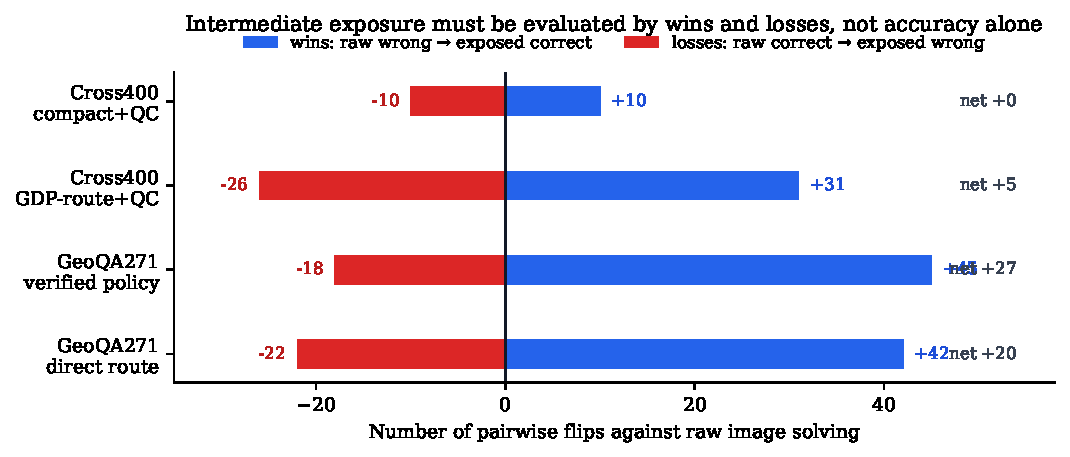
\includegraphics[width=0.88\linewidth]{figures/win_loss_decomposition.pdf}
\caption{代表性中间语言暴露策略的 pairwise win/loss 分解。仅看 accuracy 会掩盖一种方法究竟是在修正 raw 错误，还是用新错误抵消这些修正。}
\label{fig:win-loss-zh}
\end{figure}

\section{发现一：只有结构事实还不够}
在 Geometry3K-300 子集上，直接追加 GDP 自动结构没有提升 Qwen3-VL。raw image solving 为 158/300，image+GDP 为 154/300。从 pairwise 看，GDP 修正 10 个 raw 错误，但破坏 14 个 raw 原本正确的题。oracle-guided construction language 更好，达到 167/300；但它不是平铺解析结果，而是目标条件化、定理导向的语言。

\begin{table}[t]
\centering
\caption{Geometry3K-300 对比。所有结构化变体都保留原图。}
\label{tab:geometry300-zh}
\small
\begin{tabular}{lccc}
\toprule
变体 & 结构来源 & 正确数 / 总数 & 准确率 \\
\midrule
raw & 无 & 158 / 300 & 52.67\% \\
image+GDP & GDP-4B 自动解析 & 154 / 300 & 51.33\% \\
structured facts & Geometry3K oracle predicates & 161 / 300 & 53.67\% \\
construction plan & oracle predicates + 定理提示 & 167 / 300 & 55.67\% \\
\bottomrule
\end{tabular}
\end{table}

\begin{figure}[t]
\centering
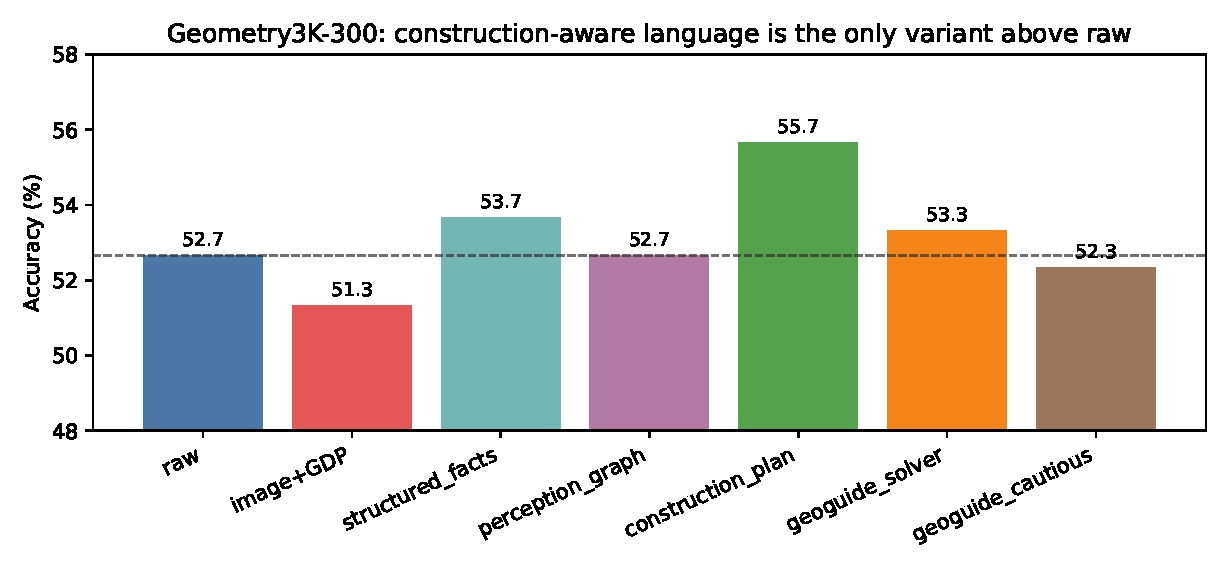
\includegraphics[width=0.82\linewidth]{figures/main_geometry300_accuracy.pdf}
\caption{结构并不会自动有用。GDP 自动结构低于 raw；construction-aware theorem language 更强。}
\label{fig:geometry300-zh}
\end{figure}

完整 Geometry3K-601 trust experiment 进一步说明了这一点。full oracle predicates 为 318/601，低于 raw 的 325/601；cautious top-6 版本与 raw 持平。这排除了一个过于简单的解释：瓶颈并不只是“缺少符号事实”。

\begin{table}[t]
\centering
\caption{Geometry3K-601 可信校准实验。oracle structure 不是 plug-and-play 的提升。}
\label{tab:trust601-zh}
\small
\begin{tabular}{lccc}
\toprule
变体 & 正确数 / 总数 & 准确率 & 解释 \\
\midrule
raw & 325 / 601 & 54.08\% & image-only baseline \\
oracle\_full & 318 / 601 & 52.91\% & 未筛选结构过多 \\
oracle\_topk6\_cautious & 325 / 601 & 54.08\% & 筛选后恢复到 raw \\
oracle\_corrupt\_trusted & 314 / 601 & 52.25\% & 错误可信事实有害 \\
\bottomrule
\end{tabular}
\end{table}

\section{发现二：定理化语言更强，但有风险}
定理路线比普通结构事实更有用，因为它更接近数学推理。在 GeoQA271 上，generated route guidance 将 Qwen3-VL 从 83/271 提高到 103/271；轻量 verified-policy 版本进一步达到 110/271。但是，direct route 仍然造成损失：22 个 raw-correct case 在 route guidance 下变错。

\begin{table}[t]
\centering
\caption{GeoQA271 route 实验。route 提高平均准确率，但仍引入 route-induced loss。}
\label{tab:geoqa271-zh}
\small
\begin{tabular}{lcccc}
\toprule
变体 & 正确数 / 总数 & 准确率 & 相对 raw 的 win & 相对 raw 的 loss \\
\midrule
image only & 83 / 271 & 30.63\% & -- & -- \\
image + generated route & 103 / 271 & 38.01\% & 42 & 22 \\
image + verified-policy route & 110 / 271 & 40.59\% & 45 & 18 \\
\bottomrule
\end{tabular}
\end{table}

这正是目前实验中最关键的矛盾：route language 的数学价值是真实存在的，但 MLLM 也会过度跟随它。单独的 FormalGeo oracle-route 检查把“路线本身有价值”这件事说得更清楚：在 200 道 FormalGeo 样本上，dataset-annotated route 将 image-only Qwen3-VL 从 58/200 提升到 83/200。由于 FormalGeo 与 GeoQA 在题目难度、标注格式和 theorem sequence 构造方式上不同，本文只把它作为辅助 sanity check，完整表格放在附录~\ref{app:formalgeo-zh}。

route generator 有时会重复某个定理，选择局部看似合理但与目标无关的定理，或者给出缺少图像支撑的路线。下游 MLLM 可能因此自信地解错问题。

\begin{figure}[t]
\centering
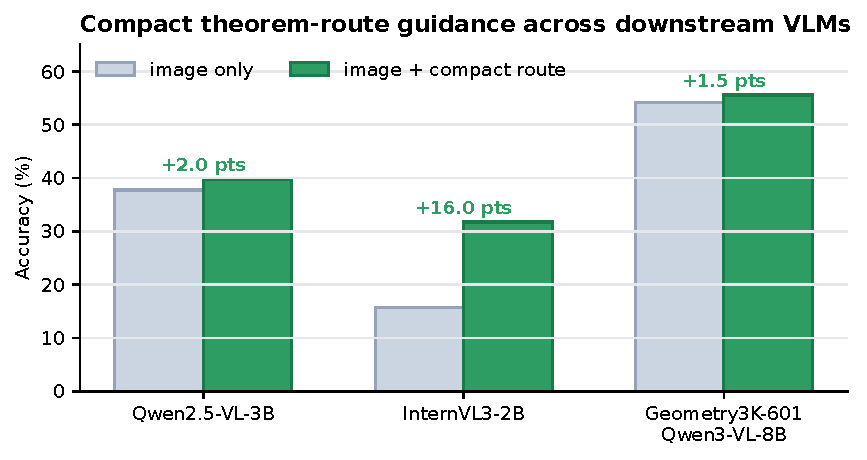
\includegraphics[width=0.86\linewidth]{figures/compact_route_multimodel_accuracy.pdf}
\caption{跨下游 VLM 的 compact-route 验证。在 PGPS9K+Geometry3K 划分上，同一 compact-route 通道同时提升 Qwen2.5-VL-3B 和 InternVL3-2B，并与早期 Geometry3K-601 上的 Qwen3-VL 结果一致。InternVL2.5-2B 本轮输出无法稳定解析为数值，因此不计入图中。}
\label{fig:compact-route-multimodel-zh}
\end{figure}

\begin{table}[t]
\centering
\caption{跨下游 VLM 的 compact-route 增益。compact route 由上游生成，并与原始图像和题干一起输入下游模型。win/loss 相对同题 image-only prediction 统计。}
\label{tab:compact-route-multimodel-zh}
\small
\begin{tabular}{lcccc}
\toprule
下游 VLM & 数据集 & Image only & Image+compact route & Win / loss \\
\midrule
Qwen2.5-VL-3B & PGPS9K+Geometry3K-400 & 151 / 400 & 159 / 400 & 26 / 18 \\
InternVL3-2B & PGPS9K+Geometry3K-400 & 63 / 400 & 127 / 400 & 72 / 8 \\
Qwen3-VL-8B & Geometry3K-601 & 325 / 601 & 334 / 601 & 27 / 16 \\
\bottomrule
\end{tabular}
\end{table}

\section{自动 GDP-route 流程中的 Compact Route}
前面的 route 实验说明定理化语言有潜力，但还不能证明最早的自动流程本身有效：
\[
\text{image}\rightarrow \text{GDP-4B structure}\rightarrow \text{route generator}\rightarrow \text{MLLM solver}.
\]
因此，我们在 400 道混合题上复测完整流程：200 道 PGPS9K 和 200 道 Geometry3K。所有 route 都由 GDP-4B 自动结构化语言生成，再输入微调后的 Qwen3-1.7B route generator。下游求解器为 Qwen3-VL-8B；所有变体都保留原始图像和题干。

\begin{table}[t]
\centering
\caption{PGPS9K 与 Geometry3K 上的跨数据集 GDP-route 验证。standard route 加质量控制对 Qwen3-VL-8B 有小幅收益；compact route 在单独跨模型实验中对较小 VLM 更有帮助。}
\label{tab:gdp-route-cross400-zh}
\small
\begin{tabular}{llccc}
\toprule
route generator & 数据集 & image only & route & route + QC \\
\midrule
\multirow{3}{*}{standard route}
& PGPS9K-200 & 104 / 200 & 101 / 200 & 103 / 200 \\
& Geometry3K-200 & 89 / 200 & 94 / 200 & 95 / 200 \\
& Overall & 193 / 400 & 195 / 400 & \textbf{198 / 400} \\
\midrule
\multirow{3}{*}{compact route}
& PGPS9K-200 & 104 / 200 & 103 / 200 & 105 / 200 \\
& Geometry3K-200 & 89 / 200 & 88 / 200 & 88 / 200 \\
& Overall & 193 / 400 & 191 / 400 & 193 / 400 \\
\bottomrule
\end{tabular}
\end{table}

\begin{figure}[t]
\centering
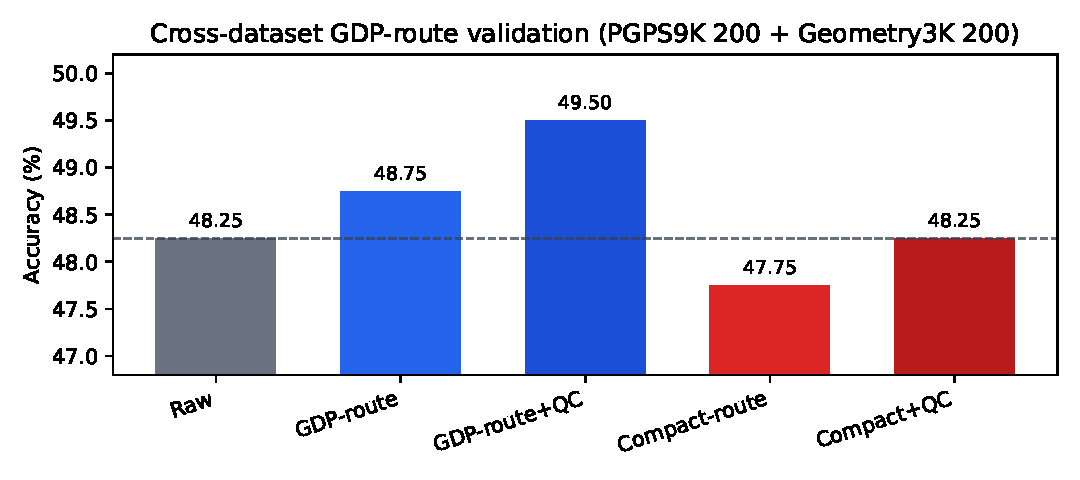
\includegraphics[width=0.86\linewidth]{figures/gdp_route_cross_dataset_400.pdf}
\caption{Qwen3-VL-8B 上的跨数据集 GDP-route 验证。standard route 加质量控制带来小幅整体提升；compact-route 结果说明 route 需要校准，而不是盲目暴露。}
\label{fig:gdp-route-cross400-zh}
\end{figure}

图~\ref{fig:compact-route-multimodel-zh} 展示了最积极的模型区间：较小 VLM 明显受益于定理级压缩。Qwen2.5-VL-3B 从 37.75\% 提升到 39.75\%，InternVL3-2B 从 15.75\% 提升到 31.75\%。这个过程不更新下游模型参数；compact route 更准确地说是一种推理时规划辅助：上游生成的 theorem planning 以文本形式提供给内部几何规划能力较弱的下游模型。表~\ref{tab:gdp-route-cross400-zh} 则说明其在强求解器上的限制。standard GDP-route 加质量控制将 Qwen3-VL-8B 的混合划分仅从 48.25\% 提升到 49.50\%，相对 raw 有 31 个 win 和 26 个 loss。收益主要来自 Geometry3K：route+QC 将 44.5\% 提升到 47.5\%。该 Qwen3-VL-8B 划分中的 compact route 并非统一更强。因此，该效果是模型相关的，而不是普适的；当强 VLM 已能直接从图像解出较多题时，收益会缩小。

因此，正确结论不是“compactness 本身解决问题”。compact route 在暴露缺失定理行动时有效，但仍然需要校准。本轮 400 题中，167/400 条 compact route 会被简单质量控制 discard，315/400 被标记为 low-confidence，平均提取长度为 5.58 个 theorem steps。这推动了级联式接口：高置信 route 直接作为 verified hint；route 级验证不足时，降级为目标绑定 theorem-equation candidates；如果两者都不可靠，则隐藏中间语言。

\begin{figure}[t]
\centering
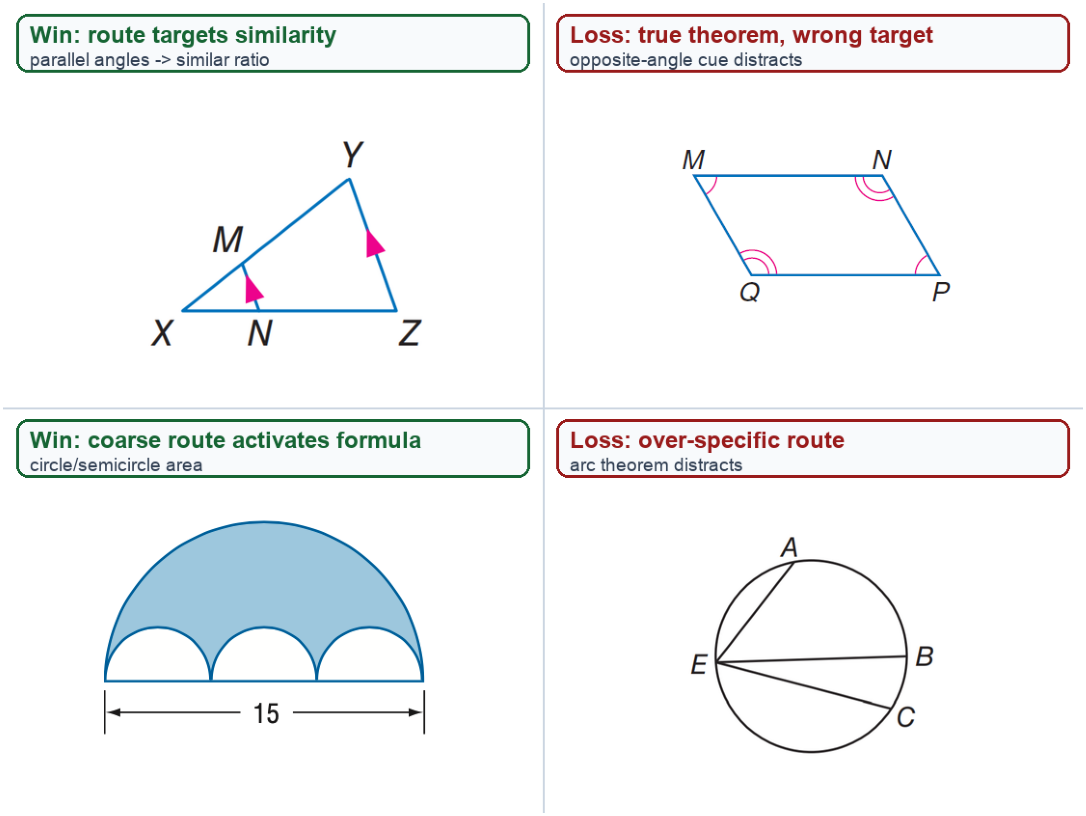
\includegraphics[width=0.88\linewidth]{figures/route_help_harm_cases.pdf}
\caption{route 带来帮助和带来伤害的代表性案例。有效 route 会把 MLLM 引向与目标直接相关的定理或计算；有害 route 往往并不“胡说”，而是绑定错了目标，或者给出过于具体但并不必要的提示，从而干扰更简单的视觉解法。}
\label{fig:route-help-harm-zh}
\end{figure}

定性地看，route-induced error 有较一致的模式。win case 中，route 通常补上了从目标量到已知量之间缺失的桥梁，例如平行线角关系指向相似比，或者圆面积公式指向阴影面积计算。loss case 中，route 不一定完全错误，而可能是目标不匹配：图中真实成立的定理未必服务于题目要求的量。GeoQA220 的粗略统计显示，角度题同时占据 direct-route win 和 loss 的多数（32 个 win 中 30 个，19 个 loss 中 14 个），因此目标类型本身不能作为绑定错误的证据。本文只用这个统计说明 route 影响集中在哪里；仍需要细粒度标注来区分定理名称错误、实体绑定错误、数值计算错误，以及模型看到 route 后产生的视觉注意力转移。

\section{从定理路线到定理-方程候选}
为什么不能只做 route 后过滤？route 是序列级对象：即使过滤掉特别长、明显重复或低置信度的 route，剩下的 route 仍可能包含局部真实但绑定错目标的定理。不过，表~\ref{tab:geoqa271-exposure-zh} 也说明，验证比格式转换更重要：verified-policy route 在同划分上强于所有 candidate 变体。因此更合理的表述是级联策略：第一，能验证 route 时优先使用 verified route；第二，当 route 级置信度不足时，将 route 拆成 theorem application，检查目标类型、实体绑定和方程后果；第三，如果 candidate 层证据也不足，退回 raw image solving。

因此，我们在 120 道 GeoQA 题上做了一个小但有信息量的 trust ablation。所有变体使用同一个 route 来源，但以不同方式交给 Qwen3-VL：直接执行路线、先批判再使用、候选定理选择，以及基于规则的 risk fallback。

\begin{table}[t]
\centering
\caption{GeoQA120 trust ablation。候选定理界面是该实验中最强变体。}
\label{tab:geoqa120-zh}
\small
\begin{tabular}{lcccc}
\toprule
变体 & 正确数 / 总数 & 准确率 & 相对 raw 的 win & 相对 raw 的 loss \\
\midrule
image only & 34 / 120 & 28.33\% & -- & -- \\
direct route & 47 / 120 & 39.17\% & 22 & 9 \\
critique-first route & 47 / 120 & 39.17\% & 23 & 10 \\
theorem candidates & 49 / 120 & 40.83\% & 24 & 9 \\
risk fallback & 45 / 120 & 37.50\% & 20 & 9 \\
\bottomrule
\end{tabular}
\end{table}

\begin{figure}[t]
\centering
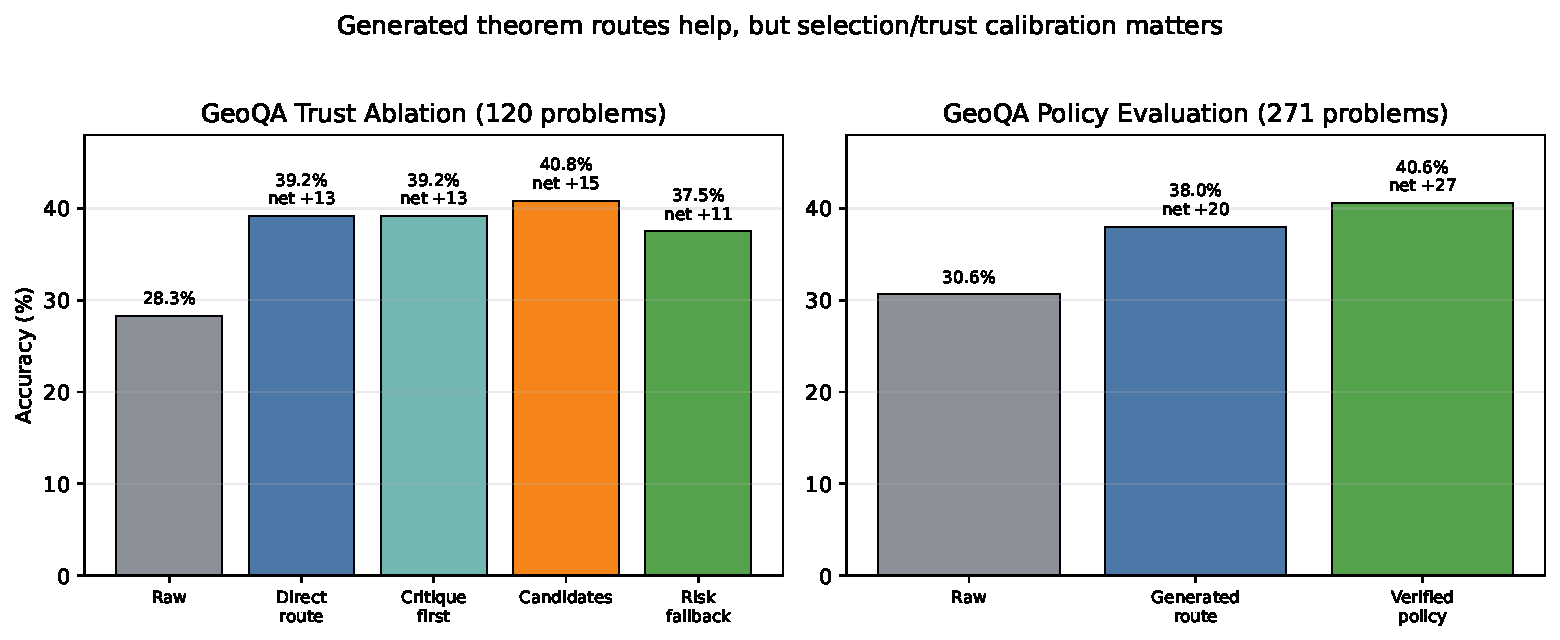
\includegraphics[width=0.88\linewidth]{figures/route_candidate_trust_summary.pdf}
\caption{GeoQA 上的 route 接口比较。候选定理选择在 120 题 trust ablation 中得到最高准确率和最高 pairwise net；verified policy 在更大的 GeoQA271 实验中也带来提升。}
\label{fig:route-candidates-zh}
\end{figure}

120 题结果说明候选选择有价值，但它并不是最终形态。我们进一步在 220 道 GeoQA 题上比较 direct route、theorem candidates、equation candidates 和 theorem+equation hybrid candidates。结果显示，单独的定理名候选会丢失部分路线顺序信息，而候选方程能通过计算骨架恢复一部分有效信号。


\begin{table}[t]
\centering
\caption{GeoQA220 candidate-grounding 实验。候选方程和 theorem+equation hybrid candidates 均超过 direct route。}
\label{tab:geoqa220-equation-zh}
\scriptsize
\setlength{\tabcolsep}{4pt}
\begin{tabular}{lccccc}
\toprule
变体 & 正确数 / 总数 & 准确率 & 相对 raw 的 win & 相对 raw 的 loss & 相对 route 净变化 \\
\midrule
image only & 69 / 220 & 31.36\% & -- & -- & -- \\
route direct & 82 / 220 & 37.27\% & 32 & 19 & -- \\
theorem candidates & 80 / 220 & 36.36\% & 34 & 23 & -2 \\
equation candidates & 84 / 220 & 38.18\% & 32 & 17 & +2 \\
hybrid candidates & \textbf{86 / 220} & \textbf{39.09\%} & \textbf{36} & 19 & \textbf{+4} \\
\bottomrule
\end{tabular}
\end{table}

\begin{figure}[t]
\centering
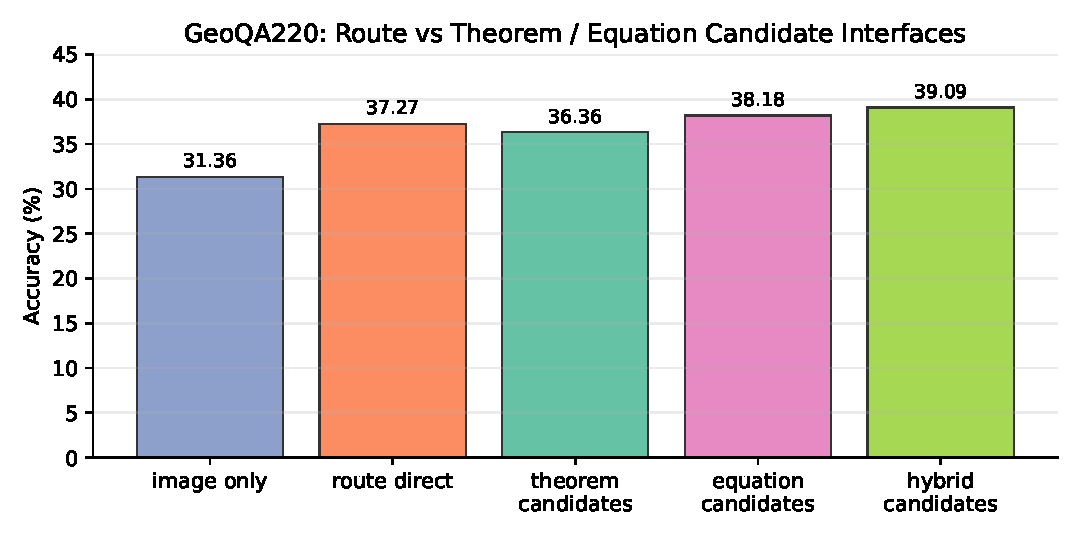
\includegraphics[width=0.86\linewidth]{figures/geoqa220_equation_candidates.pdf}
\caption{GeoQA220 candidate-grounding 结果。候选方程超过 direct route，theorem+equation hybrid candidates 表现最好。}
\label{fig:geoqa220-equation-zh}
\end{figure}


hybrid candidates 表现最好：相对 raw 的 pairwise net 为 +17，相对 direct route 的 pairwise net 为 +4。这说明更有用的单位不是单独的 theorem name，而是目标绑定的 theorem-equation pair。定理提供语义方向，方程提供可计算约束，两者组合比单独路线或单独定理候选更稳。但这个比较仍然只是 candidate interface 的 lower-bound 测试，而不是 oracle upper bound：GeoQA220 中所有 candidates 都由同一个 generated route source 转换而来，因此候选池仍受 route generator 质量约束。

为了避免在不同 GeoQA 子集上比较不同接口，我们又把这些暴露方式放回同一个 271 题划分上复测。结果改变了本文解释重点：可靠性控制比 candidate 格式更重要。equation 和 hybrid candidates 仍然优于 direct route，但 verified-policy route 仍然最好。theorem-only candidates 反而弱于 direct route。这说明 candidates 本身不是万能格式；它们的作用是让不确定的 route 信息更容易被检查、拒绝或部分使用。

\begin{table}[t]
\centering
\caption{GeoQA271 同划分暴露对比与 gate ablation。可靠性控制是当前最强干预：verified-policy route 超过所有 candidate 变体，而 strict gate 过于保守。equation 和 hybrid candidates 仍优于 direct route，说明它们更适合作为验证不足时的安全降级，而不是 verification 的替代品。}
\label{tab:geoqa271-exposure-zh}
\scriptsize
\setlength{\tabcolsep}{3pt}
\begin{tabular}{lccccc}
\toprule
变体 & 正确数 / 总数 & 准确率 & 相对 raw 的 win & 相对 raw 的 loss & 相对 route 净变化 \\
\midrule
image only & 83 / 271 & 30.63\% & -- & -- & -- \\
route direct & 103 / 271 & 38.01\% & 42 & 22 & -- \\
strict verified route & 86 / 271 & 31.73\% & 26 & 23 & -17 \\
cascade route candidate raw & 91 / 271 & 33.58\% & 30 & 22 & -12 \\
verified-policy route & \textbf{110 / 271} & \textbf{40.59\%} & 45 & 18 & \textbf{+7} \\
theorem candidates & 99 / 271 & 36.53\% & 42 & 26 & -4 \\
equation candidates & 107 / 271 & 39.48\% & 43 & 19 & +4 \\
hybrid candidates & 108 / 271 & 39.85\% & \textbf{46} & 21 & +5 \\
\bottomrule
\end{tabular}
\end{table}

这也意味着，candidate interface 只是 lower-bound 测试，而不是上界：GeoQA 的 candidates 都是用实验协议中描述的规则抽取器从同一个 generated route source 转换而来，因此候选池既受 route generator 质量约束，也受固定 theorem/equation 模板表约束。附录~\ref{app:formalgeo-zh} 中的 FormalGeo oracle-route 结果不是 GeoQA 上界，但它强化了一个定性事实：可靠 theorem route 可以有价值。更强的评测仍然需要在同一目标数据集上从标注 theorem sequence 构造 oracle candidates，并训练直接输出 theorem-equation pairs 的候选生成器。

两个 gate ablation 进一步说明了权衡关系。strict verified route 比 verified-policy 更保守：超过六步的 route 会被拒绝，同一定理重复三次及以上会被标记为风险，定理类型必须与推断出的目标类型匹配；当 route 使用 parallel、perpendicular/right-triangle 或 similar-triangle 相关定理时，解析事实中还必须出现对应前提谓词。若这些严格检查不通过，route 会被隐藏。cascade 版本使用同一个 strict gate：高置信 route 直接暴露，中置信 route 降级为 hybrid candidates，低置信 route 退回 raw image solving。这能避免部分坏 route，但也丢掉太多有用规划信号。因此，当前最好的 policy 不是最严格的 policy，而是在保留足够 route 信号的同时，用置信度和风险提示校准 MLLM 的使用方式。

\section{为什么候选暴露是安全接口}
本文引入 candidate exposure，并不是因为它在当前实验中超过 verified route，而是因为当 route 级验证不可用或不确定时，direct route 非常脆弱。定理-方程候选界面改变了 route generator 和 MLLM 之间的计算契约。

\begin{itemize}[leftmargin=*]
\item \textbf{从断言变成选择。} route 说“使用这个定理”；candidate list 说“选择前提与目标和已知条件匹配的定理”。
\item \textbf{从跟随序列变成目标绑定。} 模型必须判断某个定理是在求角、求长度、求比值还是求面积。
\item \textbf{从相信变成验证。} 错误候选可以被拒绝，而不必拒绝整个中间语言通道。
\item \textbf{从定理名到计算。} 候选方程要求被选定理实例化为具体数值关系，使中间语言更接近可执行数学。
\end{itemize}

这个视角更接近 formal geometry solver 中的 theorem application：定理应用需要把定理前提匹配到已知事实，并把定理变量绑定到图中实体。它也解释了为什么简单 critique prompt 更弱：让模型“谨慎一点”并没有给出明确的替代动作空间，而定理-方程候选选择给出了。

\section{失败模式与适用范围}
当前结果的主要局限在于：GeoQA 的 candidate list 仍然是从 generated route 转换而来，而不是由完整训练的 theorem-equation selector 直接生成。这个设置是有意为之的压力测试，但也意味着下游候选池仍受到上游 route 质量的约束。如果 GDP-style parsing 漏掉关键关系或产生幻觉关系，定理-方程候选列表仍可能不完整或误导。因此，GeoQA 结果应被理解为：在固定 generated-route source 下，暴露格式本身有帮助；而不是 theorem-equation candidate 的性能上限。FormalGeo oracle-route 检查说明可靠 route annotation 可能有用，但它还不是 GeoQA oracle theorem-equation candidate。更强的评测需要从标注 theorem sequence 构造 oracle candidates，并训练直接输出 theorem-equation pairs 的候选生成器。

评测覆盖也表明，exposure policy 必须同时按数据集和模型区分。Geometry3K、PGPS9K 和 GeoQA 的标注形式、图像分布和题型并不一致；Qwen3-VL-8B、Qwen2.5-VL-3B 和 InternVL3-2B 对 route text 的反应也不同。compact route 在下游模型缺少足够几何规划能力时最有价值，但 route-induced loss 仍然存在。因此，部署时应按数据集、模型、目标类型和 route 接受状态报告结果，并在有 oracle theorem labels 的数据上对比 generated candidates 与 oracle candidates。

\section{方法启示：目标绑定 verifier}
这些结果指向一个明确的系统架构：route-first selective exposure with candidate fallback。输入为 image、question、choices 和 GDP-style structure。系统首先对整条 generated route 打分；高置信时将 route 作为强但非 oracle 的 hint 暴露；中等置信时将 route 拆成 theorem-equation candidates；低置信时隐藏中间语言。

实际可用的候选级 verifier 应检查四类条件：定理是否匹配目标类型，绑定实体是否与题干和解析事实重合，定理必要前提是否被 parsed fact set 覆盖，以及方程后果是否直接求解目标量。本文不为这些检查指定手写固定权重。GeoQA271 同划分上的 strict rule-gate ablation 说明了原因：strict verified route 只有 86/271（31.73\%），route-candidate-raw cascade 为 91/271（33.58\%），都低于轻量 verified-policy route 的 110/271（40.59\%）。粗糙规则会拒绝有用 route，也仍可能放过弱 route。因此，可部署的级联策略应把这些检查与 learned target-binding verifier 结合：

\begin{itemize}[leftmargin=*]
\item route 高置信度：暴露 verified route 作为强提示；
\item route 中等置信度：展示定理-方程候选，让 MLLM 自己选择；
\item 低置信度：隐藏中间语言，退回 raw image solving。
\end{itemize}

下一步应使用 pairwise 标签训练并评测 verifier：raw wrong 且 route correct 标为 \textsc{use-route}，raw correct 且 route wrong 标为 \textsc{reject-route}。因此，本文原则应表述得更精确：中间几何语言在定理化、经过验证并选择性暴露时才稳定有用；candidate selection 是 route 级验证不足时的安全接口。

\section{结论}
我们的核心结论不是“结构化语言没用”，也不是“route guidance 一定有用”。证据支持更精确的说法：几何中间语言只有从描述性结构转向紧凑的定理级行动后，才更可能帮助 MLLM，但行动级语言必须选择性暴露。compact route 提升 GeoQA，并且对较小 VLM 有明显帮助，可以作为推理时定理规划辅助。它的限制是可靠性，而不是有用性。因此，更实际的方向是级联暴露：先验证 route；如果验证不足，再转化为目标绑定 theorem-equation candidates；如果置信度仍低，则隐藏中间语言并依赖 raw image solving。

\appendix
\section{FormalGeo Oracle-Route 辅助检查}
\label{app:formalgeo-zh}

表~\ref{tab:formalgeo-oracle-route-zh} 给出正文提到的 FormalGeo oracle-route 检查。它只作为定性 sanity check，而不是与 GeoQA 的直接比较，因为 FormalGeo 的题目难度、标注格式和 theorem sequence 构造方式均不同。

\begin{table}[h]
\centering
\caption{FormalGeo oracle-route 定性 sanity check。}
\label{tab:formalgeo-oracle-route-zh}
\small
\begin{tabular}{lcccc}
\toprule
变体 & 正确数 / 总数 & 准确率 & 相对 raw 的 win & 相对 raw 的 loss \\
\midrule
image only & 58 / 200 & 29.00\% & -- & -- \\
image + oracle theorem route & 83 / 200 & 41.50\% & 32 & 7 \\
\bottomrule
\end{tabular}
\end{table}

\bibliographystyle{unsrt}
\bibliography{refs}

\end{document}
